	\chapter{Ordenação de Dados}
\label{cap:ordenacao}


%\begin{itemize}
%\item importância da ordenação paralela
%\item formas de ordenação: memória e disco
%\item grandes dados: apenas disco
%\item grandes dados: problematização (tempo, limite de memória)
%\item grandes dados: sort benchmark
%\end{itemize}
%
%\begin{itemize}
%\item algoritmos de ordenação paralelos
%\item funcionamento geral
%\item condições / ingredientes / limites
%\item diferentes algoritmos para diferentes aplicações
%\item descrição de algoritmos (e diagramas): sample sort, quick sort
%
%\end{itemize}

%A ordenação é o processo de organizar elementos de uma sequência em determinada ordem, e é um dos problemas fundamentais da computação devido à sua importância teórica e prática \ite{Knuth:1998, Cormen:2001}. 
%A ordenação é utilizada por um grande número de aplicações computacionais, como compiladores e sistemas operacionais, que usam extensivamente a ordenação para lidar com tabelas e listas. Também participa 
%A ordenação participa de aplicações de computação gráfica, compressão de dados, para determinar a duplicidade de elementos, encontrar o maior valor, realizar busca contínua e encontrar the convex hull. 
%É também realizada internamente por operações SQL, em criação de índices e buscas binárias, portanto todos os sistemas que usam banco de dados se beneficiam de uma rotina eficiente de ordenação.  The construction of spatial data struc- tures that are essential in computer graphics and geographic information systems is fundamentally a sorting process
%Rotinas eficientes de ordenação também são úteis 
%Efficient sort routines are also a useful building block in implementing algorithms like sparse matrix multiplication 
%[Martin, 1971] (W. A. Martin. Sorting. ACM Comp Surv., 3(4):147–174, 1971.)


A ordenação é o processo de organizar elementos de uma sequência em determinada ordem, considerada um dos problemas fundamentais da computação devido à sua importância teórica e prática \cite{Knuth:1998, Cormen:2009}. 
A ordenação é utilizada por um grande número de aplicações computacionais, como compiladores e sistemas operacionais, que usam extensivamente a ordenação para lidar com tabelas e listas. 
A construção de estruturas essenciais em computação gráfica e sistemas de informação geográfica são fundamentalmente operações de ordenação, que também participam de aplicações como a compressão de dados. A ordenação ainda é utilizada para determinar a duplicidade de elementos, encontrar o maior valor, realizar busca contínua e por operações SQL, que internamente a utilizam na criação de índices e buscas binárias. Dessa forma, diversos sistemas e bancos de dados se beneficiariam de uma rotina eficiente de ordenação \cite{Lauterbach:2009,Satish:2009,Dean:2008}.


%A busca binária é outro exemplo de aplicação da ordenação, uma vez que necessita que a sequência de elementos esteja previamente ordenada. A ordenação também fornece uma forma fácil e rápida para solucionar o problema de verificação da duplicidade de elementos. Quando as operações são repetidas muitas vezes como, por exemplo, na busca contínua por elementos em uma massa de dados, é vantajoso ordenar a sequência primeiramente.


De forma geral, a ordenação pode ser dividida em dois grupos: ordenação interna e externa. 
A ordenação em memória interna é caracterizada pelo armazenamento de todos os registros na memória principal, onde seus acessos são feitos diretamente pelo processador. Essa ordenação é possível apenas quando a quantidade de dados é pequena o suficiente para ser armazenada em memória. 

Quando é preciso ordenar uma base de dados muito grande, que não cabe na memória principal, um outro modelo faz-se necessário, a ordenação externa.
Apesar do problema nos dois casos ser o mesmo - rearranjar os registros de um arquivo em ordem ascendente ou descendente - não é possível usar as mesmas estratégias da ordenação interna, pois o acesso aos dados precisa ser feito em memória secundária, basicamente discos, cujo tempo de acesso é várias ordens de grandeza superior ao da memória principal.  %[Ziviani 2007, Knuth 1973].

Na ordenação externa, os itens que não estão na memória principal devem ser buscados em memória secundária e trazidos para a memória principal, para assim serem comparados. Esse processo se repete numerosas vezes, o que o torna lento, uma vez que os processadores ficam grande parte do tempo ociosos à espera da chegada dos dados à memória principal para processá-los. Por esse motivo, a grande ênfase de um método de ordenação externa deve ser a minimização do número de vezes que cada item é transferido entre a memória interna e a memória externa. Além disso, cada transferência deve ser realizada de forma tão eficiente quanto as características dos equipamentos disponíveis permitam \cite{Ziviani:2007}.



\section{Ordenação Paralela}


Diversas aplicações possuem uma fase de processamento intenso, na qual é preciso ordenar uma lista de elementos. Mesmo algoritmos de ordenação sequenciais ótimos, como o \textit{QuickSort} e o \textit{HeapSort}, apresentam custo mínimo ${\cal O}(n/log \quad n)$ para ordenar uma sequência de $n$ chaves \cite{Cormen:2009}. 
Isso significa que, com o crescimento do número de elementos a ser ordenado, o tempo para realizar a ordenação aumenta de maneira não linear, o que pode ser um entrave ao processamento. 
A fim de resolver tal problema, com o surgimento do processamento paralelo, foram apresentadas versões paralelas dos algoritmos de ordenação sequenciais, com o intuito de diminuir consideravelmente o tempo de execução. A importância da ordenação têm originado estudos buscando desenvolver algoritmos de ordenação eficientes para uma grande variedade de arquiteturas paralelas \cite{Akl:1990}.

\textbf{A ordenação paralela} é o processo  de ordenação feito em múltiplas unidades de processamento, que trabalham em conjunto para ordenar uma sequência de entrada. O conjunto inicial é dividido em subconjuntos disjuntos, que são associados a uma única unidade de processamento. A sequência final ordenada é obtida a partir da composição dos subconjuntos ordenados. É um ponto fundamental do algoritmo de ordenação paralela que a distribuição dos dados a serem ordenados, em cada processo individual, seja feita de tal forma que todas as unidades de processamento estejam trabalhando e que o custo de redistribuição de chaves entre os processadores seja minimizado. 

\textbf{A ordenação paralela} é uma aplicação estudada intensivamente desde o início da computação paralela, com primeiro método \textit{Bitonic Sorting Network} proposto por Batcher \cite{Batcher:1968}. 
Estudos teóricos foram realizados inicialmente, mas testes empíricos se tornaram possíveis na década de 80 com a disponibilidade de arquiteturas vetoriais, de multiprocessadores e multicomputadores e diversas versões paralelas dos algoritmos \textit{QuickSort}, \textit{RadixSort} e \textit{MergeSort} foram propostas. 
%Os principais algoritmos estudados são o  \cite{Cole:1988}. 

O \textit{QuickSort} Paralelo foi um dos algoritmos mais estudados \cite{Deminet:1982, Quinn:1994, Sanders:1997}, mas inicialmente a divisão dos dados limitava o aumento da velocidade, independente do número de processadores utilizados. Recentemente novas implementações foram propostas, utilizando as tecnologias  de \textit{hyperthreading} disponíveis em processadores atuais para desenvolver um esquema de balanço de carga, que têm se mostrado eficiente na divisão dos dados \cite{Parikh:2008}.
Para o \textit{MergeSort} foi proposta uma versão chamada \textit{Simple Randomized Mergesort} \cite{Barve:1996, Barve:2002}, que foi o primeiro algoritmo de ordenação em disco a obter um número médio ótimo de movimentações de dados. 
 A implementação \textit{Quickmerge} proposta por Quinn combinava os algoritmos \textit{QuickSort} e \textit{MergeSort}, reduzindo significativamente a quantidade de dados movimentada \cite{Quinn:1988}. Também foram estudados algoritmos de ordenação paralela que se baseiam em uma amostra para realizar a divisão do conjunto de dados. Podem ser citados o \textit{FlashSort} \cite{Reif:1987}, o \textit{SampleSort} \cite{Huang:1983} e suas variações como o \textit{Super-Scalar SampleSort }\cite{Sanders:2004} e o \textit{Parallel Sorting by Regular Sampling} \cite{Shi:1992}.

Além disso, as propostas atuais de ordenação em grandes conjuntos de máquinas incluem os algoritmos implementados em Hadoop \textit{Sort} e \textit{TeraSort}, descritos na seção \ref{sec:benchmarks}, capazes de ordenar petabytes de informação em centenas ou milhares de nodos. 
%Outros notáveis algoritmos de ordenação são as versões paralelas do RadixSort, Quick- Sort [Blelloch 1990, Leighton 1992, Breshears 2009] e MergeSort [Cole 1988], assim como os novos algoritmos de ordenação paralelos como o PSRS ) .

%Recentemente, Sanders and Winkel  apontaram que o desempenho de uma ordenação nos processadores atuais é comumente dominada por \textit{pipeline stalls} causados por predições incorretas em desvios. Eles propuseram um novo algoritmo, chamado de super-scalar sample sort, que evita tais \textit{stalls} eliminando desvios  condicionais. 


Com tamanha variedade de algoritmos e arquiteturas, diversas soluções podem ser consideradas ao implementar um algoritmo de ordenação em ambiente paralelo. Cada uma delas atende um cenário, tipo de entrada, plataforma ou arquitetura particulares. Dessa forma, ao desenvolver algoritmos de ordenação paralela, é importante ter em mente certas condições que interferem no desempenho final do algoritmo, relacionadas tanto ao ambiente de implementação, quanto ao conjunto de dados que deve ser ordenado. As principais questões a serem analisadas são \cite{Kale:2010}:

\begin{itemize}
\item \textbf{Habilidade de explorar distribuições iniciais parcialmente ordenadas:}
Alguns algoritmos podem se beneficiar de cenários nos quais a sequência de entrada dos dados é a mesma, ou pouco alterada. Nesse caso, é possível obter melhor desempenho ao realizar menos trabalho e movimentação de dados.
Se a alteração na posição dos elementos na sequência é pequena o suficiente, grande parte dos processadores mantém seus dados iniciais e precisam se comunicar apenas com os processadores vizinhos.

\item \textbf{Movimentação dos dados:}
A movimentação de dados entre processadores deve ser mínima durante a execução do algoritmo. Em um sistema de memória distribuída, a quantidade de dados a ser movimentada é um ponto crítico, pois o custo de troca de dados pode dominar o custo de execução total e limitar a escalabilidade.

\item \textbf{Balanceamento de carga:}
O algoritmo de ordenação paralela deve assegurar o balanceamento de carga ao distribuir os dados entre os processadores. Cada processador deve receber uma parcela equilibrada dos dados para ordenar, uma vez que o tempo de execução da aplicação é tipicamente limitada pela execução do processador mais sobrecarregado.

\item \textbf{Latência de comunicação:}
A latência de comunicação é definida como o tempo médio necessário para enviar uma mensagem de um processador a outro.
Em grandes sistemas distribuídos, reduzir o tempo de latência se torna muito importante.

\item \textbf{Sobreposição de comunicação e computação:}
Em qualquer aplicação paralela, existem tarefas com focos em computação e comunicação. A sobreposição de tais tarefas permite que sejam feitas tarefas de processamento e ao mesmo tempo operações de entrada e saída de dados, evitando que os recursos fiquem ociosos durante o intervalo de tempo necessário para a transmissão da carga de trabalho.

\end{itemize}


Além das condições relacionadas à implementação do algoritmo em ambiente paralelo, existem outras condições necessárias, relacionadas principalmente ao conjunto de elementos a ser ordenado. Considerando um conjunto de $n$ chaves e  $p$ processadores,  durante a execução de qualquer algoritmo de ordenação paralela é preciso que o conjunto de chaves seja particionado em $p$ subconjuntos mutualmente exclusivos, sem nenhuma chave duplicada. É necessário ainda que todas as chaves da sequência inicial sejam mantidas, ou seja, que não se perca nenhuma chave durante a distribuição entre os processadores.

Após o conjunto estar ordenado, é preciso verificar se todas as chaves da sequência inicial foram preservadas, se todas as chaves de cada processador estão ordenadas em ordem crescente, se a maior chave no processador $p_{i}$ é inferior ou igual à menor chave no processador $p_{i+1}$ e se a saída resultante é uma sequência de chaves totalmente ordenada.


\subsection{Fluxo geral de execução da ordenação paralela}

Na execução de um algoritmo de ordenação paralela podem ser identificadas algumas tarefas principais, que todos os algoritmos precisam executar em algum momento, normalmente realizadas de forma sequencial  \cite{Kale:2010}. 
A primeira tarefa é a ordenação local, na qual as chaves em cada processador são ordenadas inicialmente  ou ordenadas em grupos.
Existe também uma fase de agrupamento, pois muitas vezes é necessário colocar as chaves em grupos, a fim de enviá-las a outros processadores ou calcular histogramas. Por fim, é preciso realizar a intercalação das chaves ordenadas em subsequências em uma sequência completa.

%visto pela perspectiva da comunicação, pode ser generalizada, uma vez que estão submetidos às mesmas limitações. 
%A fim de fazer uma generalização sobre o fluxo de controle de algoritmos de ordenação, algumas tarefas 

Os algoritmos de ordenação paralela executam tarefas similares que podem ser definidas, genericamente, como se segue: 
\begin{num_enum}
\item Realizar processamento local;
\item Coletar informações relevantes de distribuição de todos os processadores;
\item Em um único processador, inferir uma divisão de chaves a partir das informações coletadas;
\item Transmitir aos outros processadores a divisão dos elementos;
\item Realizar processamento local;
\item Mover os dados de acordo com os elementos de divisão;
\item Realizar processamento local;
\item Se a divisão de chaves foi incompleta, retornar ao passo 1;
\end{num_enum}

De acordo com essa generalização  é possível identificar pontos que se relacionam diretamente com as condições que limitam o desempenho dos algoritmos de ordenação paralela e fornecem ideias para a análise de eficiência da comunicação dos algoritmos.
Primeiro, há duas tarefas principais de comunicação: descobrir um vetor de divisão global e enviar os dados para os processadores adequados. 
Em segundo lugar, a maioria dos algoritmos têm múltiplos estágios de computação local e pode ser muito vantajoso sobrepor este processamento local e a comunicação. 
%Finalmente, se é possível realizar sobreposição entre o processamento local e a determinação do vetor de divisão, um processador pode ser reservado para o trabalho de divisão, encurtando o caminho crítico. 
A fração de  processamento local que pode ser sobreposta à comunicação necessária em um algoritmo  é um bom indicativo para comparação da escalabilidade dos algoritmos de ordenação paralela.
%ao custo para determinar a divisão e mover os dados

\section{Algoritmos de Ordenação Paralela}

Essa seção apresenta os algoritmos de ordenação paralela objetos desse trabalho: o algoritmo Ordenação por Amostragem  (\textit{SampleSort}) e o algoritmo \textit{QuickSort} Paralelo, bem como as aplicações de ordenação em Hadoop \textit{Terasort} e \textit{Sort}.  

\subsection{Ordenação por Amostragem}

O algoritmo \textit{SampleSort} ou Ordenação por Amostragem é um método de ordenação baseado na divisão do arquivo de entrada em subconjuntos, de forma que as chaves de um subconjunto $i$ sejam menores que as chaves do subconjunto $i+1$. Após a divisão, cada subconjunto é enviado a um processador, que ordena os dados localmente. Ao final, todos os subconjuntos são concatenados e formam um arquivo globalmente ordenado.

Nesse algoritmo, o ponto chave é dividir as partições de maneira balanceada, para que cada processador receba aproximadamente a mesma carga de dados. Para isso, é preciso determinar o número de elementos que devem ser destinados a uma certa partição, o que é feito através da amostragem das chaves do arquivo original. Essa estratégia baseia-se na análise de um subconjunto de dados  denominado amostra, ao invés de todo o conjunto, para estimar a distribuição de chaves e construir partições balanceadas.

Existem três tipos de estratégias de amostragem: \textit{SplitSampler}, \textit{IntervalSampler} e \textit{RandomSampler}. O \textit{SplitSampler} seleciona os $n$ primeiros registros do arquivo para formar a amostra. O \textit{IntervalSampler} cria a amostra com a seleção de chaves em intervalos regulares no arquivo. No \textit{RandomSampler}, a amostra é constituída por chaves selecionadas aleatoriamente no conjunto. A melhor estratégia de amostragem depende diretamente dos dados de entrada. O \textit{SplitSampler} não é recomendado para arquivos quase ordenados, pois as chaves selecionadas serão as iniciais, que não são representativas do conjunto como um todo. Nesse caso, a melhor escolha é o \textit{IntervalSampler} pelo fato de selecionar chaves que representam melhor a distribuição do conjunto. O \textit{RandomSampler} é considerado um bom amostrador de propósito geral [White 2009], e foi o amostrador escolhido na implementação do algoritmo Ordenação por Amostragem feito por Pinhão (2011), que foi utilizado neste trabalho.

Para criar a amostra, o \textit{RandomSampler} necessita de alguns parâmetros, como a probabilidade de escolha de uma chave, o número máximo de amostras a serem selecionadas para realizar a amostragem e o número máximo de partições que podem ser utilizadas.
O número máximo de partições é determinado pelo número de núcleos disponíveis por processador e pela quantidade de máquinas, de acordo com a equação: \mbox{$ parti \text{\c{c}} \tilde{o}es = n\acute{u}cleos \times m\acute{a}quinas$}.
Após a definição das amostras, são conhecidos os intervalos compreendidos por cada partição. As informações das partições são armazenadas em um arquivo e transmitidas para as demais máquinas por meio de cache distribuído.

O algoritmo Ordenação por Amostragem, quando implementado no modelo MapReduce no ambiente Hadoop pode ser dividido nas fases Map e Reduce.
Na fase Map os arquivos de entrada são lidos e são formados os pares (chave, valor) para cada registro presente no arquivo. 
Em seguida é definido o vetor contendo as amostras. A partir desse vetor de amostras os dados são divididos em partições. O número de partições é determinado pelo número de máquinas e núcleos de processamento. 
Por meio de cache distribuído, as informações das partições são transmitidas para as máquinas participantes e os dados particionados. Cada partição é atribuída a um processador, que executa a tarefa Reduce.

Na fase Reduce, cada processador ordena os dados localmente. Essa ordenação é realizada pelo próprio \textit{framework}, que avalia a profundidade da árvore de recursão e escolhe entre os  algoritmos \textit{QuickSort} e \textit{HeapSort}. 
Após a ordenação local os dados são enviados para a máquina mestre, na qual são concatenados e formam o conjunto final ordenado.

O balanceamento das partições, ou seja, a formação de partições com tamanhos aproximados é fundamental para o algoritmo de Ordenação por Amostragem, pois reduz a possibilidade de que um processador esteja ocioso, enquanto outro processador está sobrecarregado, situação que comprometeria o desempenho do algoritmo \cite{White:2009}.

%evita que os tempos de ordenação sejam dominados por um único processador. Em outras palavras, o equilíbrio das partições  

A Figura \ref{fig:samplesort} apresenta um exemplo de como seria a execução do algoritmo implementado no Hadoop. 
Nesse exemplo, está representada a execução do algoritmo em duas máquinas com dois núcleos cada, totalizando 4 unidades de processamento. 
Primeiramente foram lidos os arquivos e formados os pares (chave, valor) (passos 1 e 2). 
 Em seguida foram amostrados 3 valores com o \textit{RandomSampler}  (passo 3) para determinar os valores presentes nas 4 partições  (passo 4). Após formadas as partições, os dados foram distribuídos para os escravos executarem a função Reduce.  
A função Reduce ordena localmente os dados  (passo 5) e o mestre agrupa todos os valores, escrevendo o arquivo final (passo 6).

\begin{figure}[htb]
\centering
%trim left, bottom, right and top
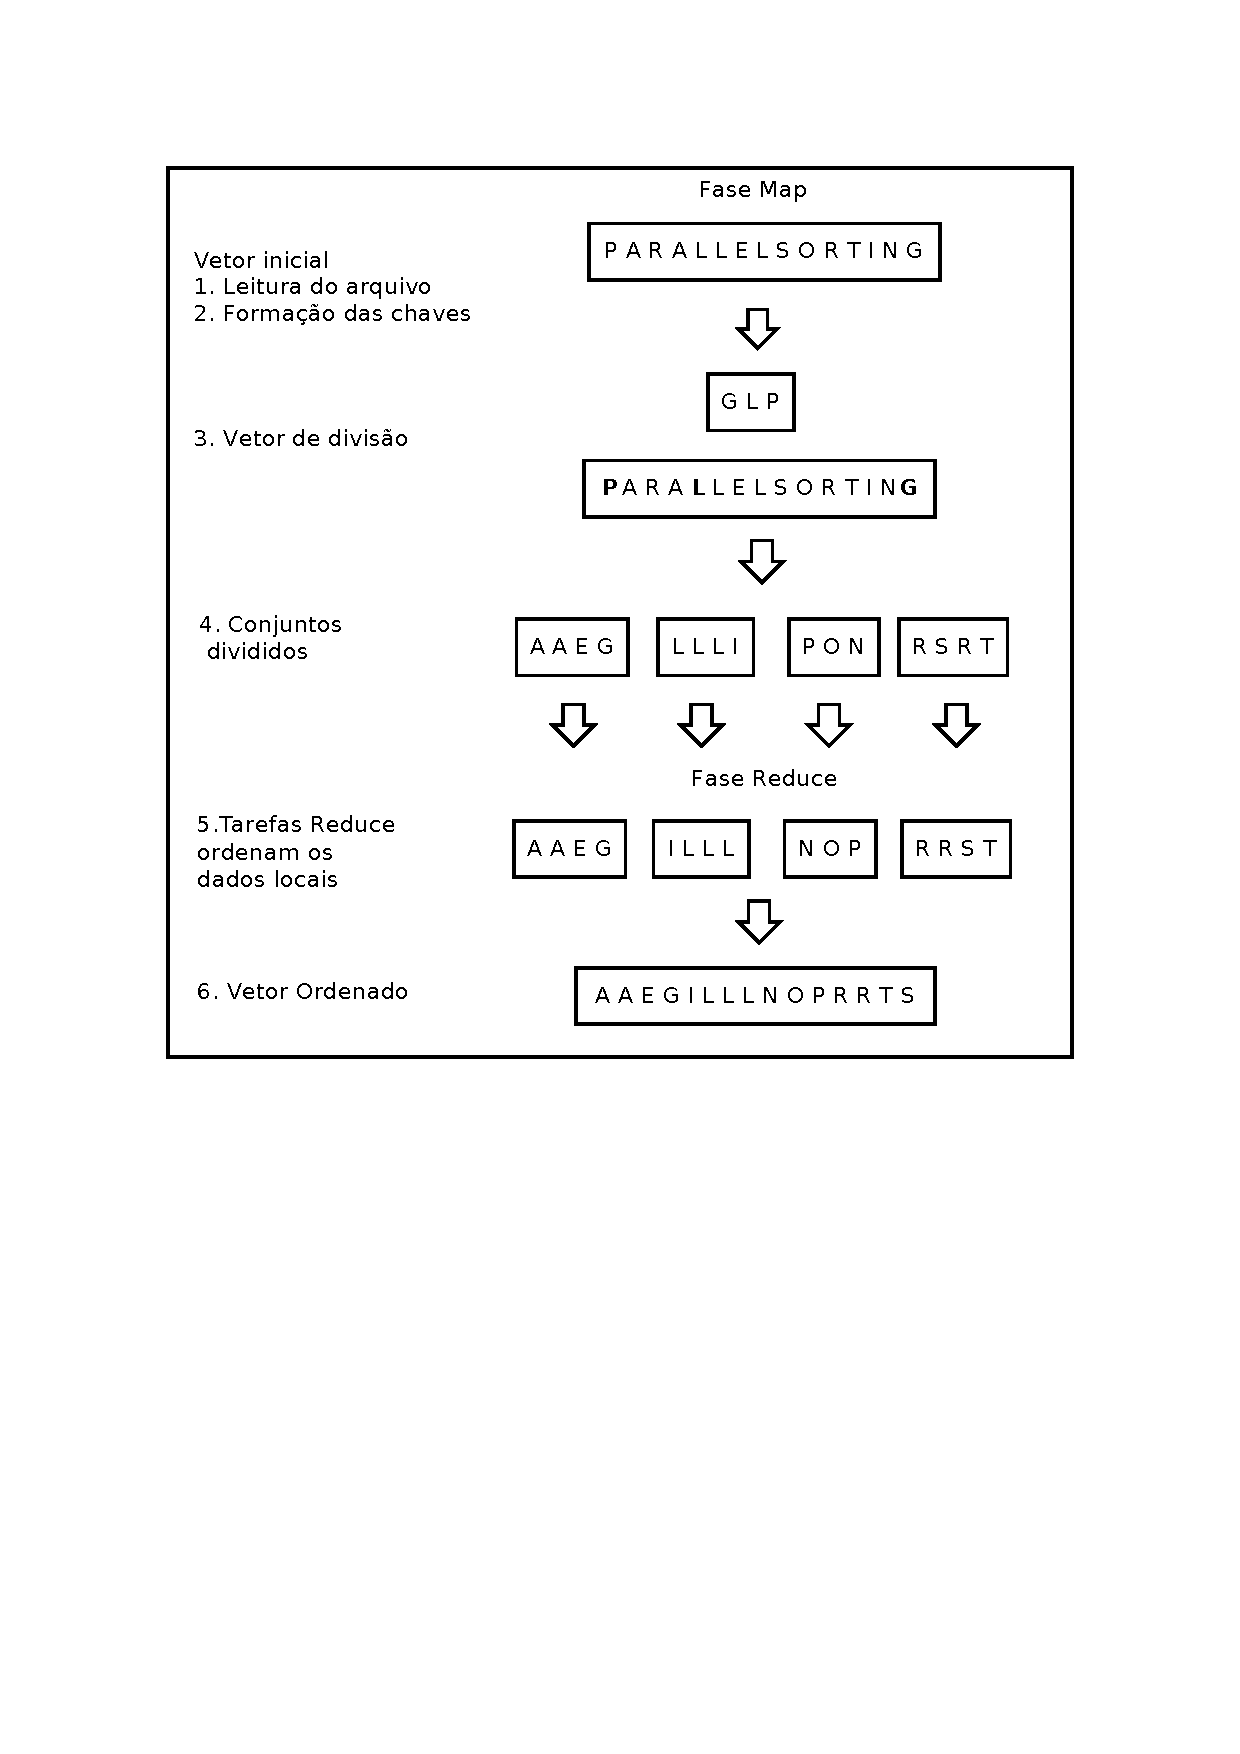
\includegraphics[trim=2cm 11cm 2cm 2cm, width=0.75\textwidth]{figuras/SampleSort.pdf}
\caption{Exemplo do algoritmo Ordenação Por Amostragem}
\label{fig:samplesort}
\end{figure}

\subsection{Quicksort}


%O algoritmo QuickSort é um método de ordenação muito rápido e eficiente, inventado por  e publicado em 1962, após uma série de refinamentos [Shustek 2009]. Ele aplica a abordagem 􏰂dividir para conquistar􏰃

O \textit{QuickSort} foi criado por Hoare em 1960 e é considerado o algoritmo de ordenação sequencial mais rápido em grande parte dos casos \cite{Cormen:2009}. É um algoritmo recursivo, que usa a estratégia Dividir para Conquistar para ordenar as chaves.
Na implementação sequencial, a estratégia é o particionamento recursivo da sequência de entrada utilizando um elemento como pivô.  
Após a escolha do elemento pivô, a lista é dividida em duas sublistas, uma contendo elementos iguais e menores que o pivô,  e outra contendo elementos maiores.
Em cada sublista é escolhido um novo pivô e o processo se repete, até que cada lista contenha apenas um elemento.  Ao final obtém-se um conjunto com elementos ordenados. 

Em geral, a complexidade da versão sequencial do algoritmo \textit{QuickSort} é ${\cal O}(n \times log \quad n)$, mas em uma situação em que a entrada de dados seja um  conjunto ordenado ou quase ordenado o desempenho do \textit{QuickSort} pode ser comprometido, caso o pivô seja escolhido nas extremidades do conjunto, pois o tamanho das partições será muito desigual. Nesse cenário a complexidade do algoritmo pode chegar a ${\cal O}(n^2)$, assim o melhor caso será quando os conjuntos de dados tiverem tamanhos próximos após o particionamento.
 
 % PARALELO
 
 
A estratégia de dividir para conquistar é naturalmente extensível à paralelização, por isso o \textit{QuickSort} é um dos algoritmos mais promissores de ordenação paralela do ponto de vista da escalabilidade.
%pois após a divisão das chaves para os processadores a ordenação em cada um deles é independente, 
Existem várias implementações paralelas do \textit{QuickSort}, por exemplo: \textit{Quinn's QuickSort, Hyper QuickSort, Sanders QuickSort} e  \textit{Grama QuickSort} \cite{Quinn:1994, Sanders:1997}. Apesar das variações, todas as implementações se baseiam em um conjunto de processadores, um mecanismo de escolha do pivô e uma lista de chaves para nelas operarem. A saída dos algoritmos é uma sequência de chaves globalmente ordenadas. 

A versão paralela do \textit{QuickSort} utiliza pivôs para realizar o particionamento recursivo no conjunto de processadores que interagem. A questão do balanceamento de carga, fundamental ao desempenho do algoritmo é mantida pela semântica da seleção do pivô [Kale e Solomonik 2010]. Inicialmente tem-se um conjunto de chaves e $p$ processadores, sendo um mestre e os demais escravos. Em seguida é feita a escolha do pivô e o mestre envia esse valor para os processadores escravos. Cada processador divide suas chaves em dois grupos: elementos maiores e elementos menores que o pivô. 
Para que  a distribuição dos conjuntos seja balanceada, são contabilizados os totais de elementos maiores e menores e com essa informação o mestre é capaz de definir o número de processadores que deve receber chaves menores e o número de processadores que deve receber chaves maiores que o pivô, além do número médio de chaves que cada processador deve receber. 

No \textit{QuickSort} Paralelo, todas as chaves serão movidas entre os processadores durante a execução do algoritmo. No entanto, a latência de comunicação das mensagens aumenta apenas com o crescimento do número de processadores. Com isso a versão paralela do \textit{QuickSort} está sujeita a menor \textit{overhead} de latência de comunicação que as versões paralelas do \textit{RadixSort} e Ordenação por Amostragem. A complexidade da versão paralela do \textit{QuickSort} é ${\cal O}((n/p) \times log(n/p))$, pois o conjunto de $n$ elementos é divido entre os $p$ processadores.  

%, tendo-se p processadores, pode-se dividir a lista de n elementos em p sublistas em um tempo O(n). Após isso, a ordenação será concluída em um tempo .
 
O \textit{Quicksort} Paralelo apresenta vantagem em relação a outros algoritmos de ordenação paralela pois 
não necessita de sincronização. Cada sublista gerada é associada a um único processo, que não precisa se comunicar com os demais porque seus dados são independentes. 

%%% EXEMPLO
%A Figura 4.3 mostra três etapas de particionamento de um vetor de dez chaves inteiras. A primeira linha mostra os dados originais; a segunda mostra os dados após o vetor ter sido particionado; e a terceira mostra como cada uma das duas partições, a partir da segunda linha, seria particionada. As caixas encapsulam as partes do vetor que precisam ser ordenadas.

	
 \subsection{Ordenação no ambiente Hadoop}
\label{sec:benchmarks}
A ordenação de dados é uma das cargas de trabalho mais consideradas pelos \textit{benchmarks} em geral, que buscam, a partir de uma entrada desordenada, obter uma saída ordenada e avaliar o desempenho do algoritmo que realizou a ordenação.

% O \textit{framework} Hadoop disponibiliza diversos programas que podem ser facilmente executados, dentre os quais se destacam o \textit{Sort} e o \textit{TeraSort}.
O \textit{Sort} é um \textit{benckmark} criado por Jim Gray em 1998, e hoje é um dos mais conhecidos na ordenação de dados \cite{Gray:1998}. 
Consiste em um conjunto de seis \textit{benchmarks}, cada um com as suas regras, que medem os tempos para ordenar diferentes números de registros e se diferem principalmente nas métricas de avaliação. 
As principais categorias dos \textit{benchmarks Sort} são a \textit{MinuteSort} e a \textit{GraySort}. A categoria \textit{MinuteSort} deve ordenar a maior quantidade dos dados em um minuto e a \textit{GraySort} deve ordenar mais que 100 terabytes em pelo menos uma hora \cite{White:2009}. Ainda existem as categorias \textit{PennySort}, \textit{JouleSort}, e os descontinuados  \textit{DatamationSort} e \textit{TeraByte Sort}. 
Em cada categoria de ordenação, existem duas classificações, de acordo com o tipo de registro a ser ordenado: \textit{Daytona} e \textit{Indy}. Os participantes da categoria \textit{Daytona} são códigos de ordenação de propósito geral, e os participantes da \textit{Indy} devem ordenar apenas registros de 100 bytes, sendo os primeiros 10 bytes reservados para a chave e o restante compõe o valor do elemento a ser ordenado.


No Hadoop, o \textit{Sort} é uma aplicação MapReduce, composta de três etapas: gerar dados aleatórios, realizar a ordenação e validar os resultados.
A geração de dados aleatórios é feita com o programa \textit{RandomWriter}. Ele executa dez tarefas MapReduce por nó, e cada função Map gera aproximadamente 1GB,  totalizando 10GB de dados binários aleatórios. 
É possível determinar o número de dados e as configurações para os tamanhos das chaves e valores a serem gerados alterando algumas configurações do \textit{RandomWriter}.
No segundo passo é realizada uma ordenação parcial dos dados de entrada e  o resultado é escrito em um diretório de saída. 
O passo final é validar os resultados obtidos pela ordenação dos dados realizada pelo \textit{Sort}, através do programa \textit{SortValidator}, que realiza uma série de verificações nos dados ordenados e nos não ordenados para confirmar se a ordenação foi realizada corretamente. 
%:
%\begin{verbatim} %SUCCESS! Validated the MapReduce framework's 'sort' successfully. \end{verbatim}
Esse programa é muito útil para verificar o desempenho do sistema como um todo, uma vez que todo o conjunto de dados é transferido através da aplicação.

%
%
%O Sort é um dos mais conhecidos 
%Os benchmarks relacionados ao Sort possuem uma aplicação MapReduce, que realiza uma ordenação parcial dos dados de entrada, e são constituídos de três passos:
%1. Geração de dados: gera dados aleatórios a serem ordenados;
%2. Ordenação dos dados: ordena os dados gerados pelo passo 1;
%3. Validação de dados: vno passo 2.
%
%

%Hadoop comes with a MapReduce program that does a partial sort of its input. It is very useful for benchmarking the whole MapReduce system, as the full input dataset is transferred through the shuffle. The three steps are: generate some random data, perform the sort, then validate the results.
%First we generate some random data using RandomWriter. It runs a MapReduce job with 10 maps per node, and each map generates (approximately) 10 GB of random binary data, with key and values of various sizes. You can change these values if you like by setting the properties test.randomwriter.maps_per_host and test.random write.bytes_per_map. There are also settings for the size ranges of the keys and values; see RandomWriter for details.

%This command runs the SortValidator program, which performs a series of checks on the unsorted and sorted data to check whether the sort is accurate. It reports the out- come to the console at the end of its run:
%SUCCESS! Validated the MapReduce framework's 'sort' successfully.



O \textit{TeraSort} é outra aplicação de destaque para ordenação de dados com Hadoop, criada por Owen O' Malley [O'Malley e Murthy 2009], com o intuito de participar da competição \textit{Sort} [Gray 1998]. Em 2009, o \textit{TeraSort} foi o campeão dessa competição em duas categorias: \textit{MinuteSort} ao ordenar 500 GB em 59 segundos, utilizando um \textit{cluster} com 1.406 nodos; e \textit{GraySort} ordenando 100 TB em 173 minutos em um \textit{cluster} com 3.452 nodos. A escalabilidade da solução foi provada pela ordenação de 1 PB em 975 minutos (equivalente a 16,25 horas) em 3.658 nodos.
O \textit{TeraSort} consiste de três algoritmos, que são responsáveis pela geração dos dados, ordenação e validação. 

\textit{Teragen} é o programa padrão para geração dados para a ordenação com \textit{Terasort}.
Nele o número de registros gerados é um parâmetro definido pelo usuário, assim como o número de tarefas Map a serem realizadas. O programa divide o número desejado de registros pelo número de tarefas Map, e atribui a cada tarefa Map um intervalo de chaves para a geração de um arquivo. Cada tarefa Map corresponde a um arquivo de saída, assim os dados gerados são divididos em diversos arquivos. Deste modo, se existem duas tarefas Map, são escritos dois arquivos, cada um contendo metade das chaves geradas. 
Os registros gerados têm um formato específico: uma chave, um id e um valor. As  chaves são caracteres aleatórios do conjunto \mbox{ `` '' .. ``$\sim$''}. O id é um valor inteiro que representa a linha, e o valor consiste de 70 caracteres de `A' a `Z'. 

\textit{TeraSort} é uma espécie MapReduce padrão, mas apresenta um particionador personalizado que usa uma lista ordenada de $ N-1 $ chaves amostradas que definem a faixa de chaves para cada função Reduce. 
Em particular, todas as chaves tal que $amostra [i-1] \le chave < amostra[i] $ são enviadas para a função \textit{i}. 
Isto garante todas as chaves da saída $i$ sejam menores que as da saída $i + 1$ .
Há também um formato de entrada e saída, \textit{TeraOutputFormat}, que é utilizado	 por todas as três aplicações  para ler e gravar os arquivos de texto no mesmo formato. 

%todas as chaves menores que a amostra i e maiores ou iguais a amostra i + 1 são enviadas ao processador i. 


\textit{TeraValidate} garante que a saída está totalmente ordenada. A aplicação cria uma função Map para cada arquivo no diretório de saída, que se certifica que cada chave é  menor ou igual à anterior. O Map também gera registros com a primeira e última chave de cada arquivo. Em seguida, a função Reduce lê tais registros e garante que a primeira chave de um arquivo é maior do que a última chave do arquivo anterior. Caso alguma chave seja encontrada fora de ordem, ela é escrita em um  arquivo de saída do Reduce, caso nenhuma chave esteja fora de ordem, não há saídas na função Reduce.


%TeraGen generates output data that is byte-for-byte equivalent to the C version including the newlines and specific keys. It divides the desired number of rows by the desired number of tasks and assigns ranges of rows to each map. The map jumps the random number generator to the correct value for the first row and generates the following rows. For the final run, I configured TeraGen to use 1,800 tasks to generate a total of 10 billion rows in HDFS, with a block size of 512 MB.
%TeraSort is a standard MapReduce sort, except for a custom partitioner that uses a sorted list of N−1 sampled keys that define the key range for each reduce. In particular, all keys such that sample[i−1] <= key < sample[i] are sent to reduce i. This guarantees that the output of reduce i are all less than the output of reduce i+1. To speed up the partitioning, the partitioner builds a two-level trie that quickly indexes into the list of sample keys based on the first two bytes of the key. TeraSort generates the sample keys by sampling the input before the job is submitted and writing the list of keys into HDFS. I wrote an input and output format, which are used by all 3 applications, that read and write the text files in the right format. The output of the reduce has replication set to 1, instead of the default 3, because the contest does not require the output data be replicated on to multiple nodes. I configured the job with 1,800 maps and 1,800 reduces and io.sort.mb, io.sort.factor, fs.inmemory.size.mb, and task heap size sufficient that transient data was never spilled to disk other at the end of the map. The sampler used 100,000 keys to determine the reduce boundaries, although as can be seen in Fig- ure 14-21, the distribution between reduces was hardly perfect and would benefit from more samples. You can see the distribution of running tasks over the job run in Fig- ure 14-22.
%
%TeraValidate ensures that the output is globally sorted. It creates one map per file in the output directory, and each map ensures that each key is less than or equal to the previous one. The map also generates records with the first and last keys of the file, and the reduce ensures that the first key of file i is greater than the last key of file i−1. Any problems are reported as output of the reduce with the keys that are out of order.
